\documentclass[12pt]{article}
\usepackage{lingmacros}
\usepackage{tree-dvips}
\usepackage{enumitem}
\usepackage{cite}
\usepackage{graphicx}
\usepackage{float}
\usepackage{caption}
\begin{document}

\section*{Cu Exchange and Siting Preference in Zeolites: the Influence of the framework topology}

Zhenghang Zhao\textsuperscript{1} ..... William F. Schneider\textsuperscript{1,*}

{\small
\enumsentence{Department of Chemcial and Biomolecular Engineering, University of Notre Dame, Notre Dame, IN, 46556}
* Corresponding Author: wschnei1@nd.edu 
}                     

\subsection*{Abstract}

Cu-exchange SSZ-13 has been confirmed active for the selective catalytic reduction (SCR) of NO\textsubscript{X} with NH\textsubscript{3} in diesel engine aftertreatment system. The nature of the Cu siting in the SSZ-13 is essential to the redox cycle and the Cu pairability. However, SSZ-13 is a zeolite material with Chabazite topology, which contains only one symmetry-distinct tetrahedral-site and 3-dimensional pore openings. The influence of the zeolite topology in the Cu exchange is still unclear. In this work, we performed Plane-wave-based Density Functional Theory supercell calculations to investigate the Cu exchange and siting preference in 4 different frameworks. We choose FER, AEI and TON to be compared with CHA to address different features of the framework topology including the pore dimensionality, the number of distinct T-site, the double-six-ring building unit, etc. Our results show the similarity and difference between zeolite frameworks\cite{Nobody06}

\subsection*{Introduction}
\subsubsection*{Objectives}
We compare the types of Cu sites and exchange energetics, compositional phase diagrms among CHA, AEI, FER and TON in order to 1) understand the influence of zeolite topology, similarities and differences between different framework. 2) Propose a design strategy to guide the choice of zeolite framework to achieve specific catalytic purposes.

\subsubsection*{Justification}
\begin{enumerate}
\item Cu SSZ-13 is a ion-exchange zeolite material that has a chabazite framework. implemented as the on-board selective catalytic reduction (SCR) catalysts in diesel engine aftertreatment system. The whole SCR cycle include the pairing and oxidation of 2 Cu\textsuperscript{+} clusters to a Cu\textsuperscript{2+} oxo cluster, and the reduction of the Cu\textsuperscript{2+} back to Cu\textsuperscript{+}. Thus, the nature of the Cu$^{+}$ and Cu$^{2+}$ are essential to learn the relation between the SCR mechanism and the framework topology, Si/Al ratio, etc.
\end{enumerate}

\begin{enumerate}
\item In SSZ-13 it is now well established that Cu2+ exchanges into the framework at proximal pairs of charge-compensating framework Al within a six-membered ring (6MR) to create Z2Cu sites and at isolated framework Al to form ZCu$_{2+}$OH sites.\cite{Paolucci2016}  Experiments and calculations are consistent with preferential population of the former sites before the latter. By combining this insight with models for the distribution of Al on the SSZ-13 framework, it is possible to create a composition phase diagram for relative fractions of Z2Cu and ZCuOH in SSZ-13.\cite{Paolucci2016}
\end{enumerate}

\begin{enumerate}
\item Construction of the composition phase diagram for SSZ-13 is facilitated by the high symmetry of the CHA lattice, resulting in only one symmetry-distinct tetrahedral site. In this work, we explore extending this  methodology to lower symmetry frameworks, with a particular emphasis on AEI, FER and TON, chosen because they represent different numbers of symmetry-distinct T-site, different pore dimensionality, different building units.
\end{enumerate}

\subsubsection*{Background}
\begin{enumerate}
\item SSZ-13 is on-board catalyst for SCR
\end{enumerate}
Zeolite, a type of mesoporous aluminosilicate materials, are mainly used as catalyst in petrolieum engineering or oil refining reactions. Cu-exchange SSZ-13
 
\begin{enumerate}[resume]
\item The Cu exchange and siting have been investigated both experimentally and theoretically
\end{enumerate}

\begin{enumerate}[resume]
\item Other emerging frameworks for SCR, and the uncertainty of the zeolite topology
\end{enumerate}

\begin{enumerate}[resume]
\item Our approach in this paper
\end{enumerate}

\begin{enumerate}[resume]
\item What's new in this work
\end{enumerate}

\subsection*{Computational Methods}

CHA, FER, AEI and TON conventional unit cells were determined from the IZA structure. A 1 $\times$ 1 $\times$ 1 supercell was constructed for CHA, FER and AEI, while a 1$\times$ 1$\times$ 2 supercell was constructed for TON. For each framework, Si was  substituted by Al to cover all available T-sites. H, Cu and CuOH were placed in all possible locations in each T-site for each framework. A enumeration code was established to enumerate all possible T-site pairs for each framework, and 2 Si were substituted by Al. DFT simulations were performed using the Vienna ab-initio Simulation Package (VASP). Spin-polarized DFT energies were determined within the generalized gradient approximation and projector-augmented wave description of core states. Calculations are conducted with a 72 T-site supercell. Construction of relative energy diagrams followed the previous procedures [1] and was further normalized to mole of exchanged Cu ions.



\subsection*{Guidance to the reader}
Here, we compute the DFT exchange energies for Z$_{2}$Cu and ZCuOH in CHA, AEI, FER and TON. We build a linear model to .....

\subsection*{Results and Disscussions}
\begin{enumerate}
\item The types of exchange sites in zeolites, Z and Z2 sites
\end{enumerate}

When Cu is exchanged in the framework, it may maintain either +1 or +2 state, which resulting in ZCu, ZCuOH and Z$_{2}$Cu forms. Here, Z indicates a frameworked Al site. These sites form in exchange with the bronsted-acid sites (ZH and Z$_{2}$H$_{2}$) that are pre-existed in the framework.

FER has a two-dimensional window structure formed from both 10- and 8-membered-ring channels, and TON has a one-dimensional window structure formed from 10-membered-ring channels. AEI has a three-dimensional window structure formed from 8-membered-ring, but a different stacking of the double 6-ring building unit s from CHA (Figure 1). The consequence of different dimensional window structure is some Cu+ pairs are blocked by small-number-ring walls. We create statistical models using Monte Carlo simulation for Cu\textsuperscript{+} ion pairability. We apply pairing rules using diffusion radius of 9 Å, and window connectivity. The results show when using the diffusion radius as pairing rule, all 4 zeolite frameworks predict the same value of pairable Cu+, because the total number of unique pairs in each framework is nearly the same. When using window connectivity as the pairing rule, AEI and CHA have higher fraction of pairable Cu\textsuperscript{+} compared to FER, while TON predicts significantly less fraction of pairable Cu\textsuperscript{+} than other frameworks do (Figure 2). The reason is that FER and TON are 2- and 1-dimensional framework. When at the reduction-limited regime, active Cu+, inactive Cu+ and Cu\textsuperscript{2+} present in SCR, and our model recovers the fraction of active Cu\textsuperscript{+}. It indicates the dimensionality of zeolite framework controls the fraction of pairable Cu\textsuperscript{+} during SCR oxidation half-cycle. This is consistent with preliminary experimental results that Cu-FER shows slower rates compared to CHA at high O\textsubscript{2} pressure limit.


\begin{enumerate}[resume]
\item ZH exchange energies and siting locations
\end{enumerate}

\begin{figure}[H]
\centering
  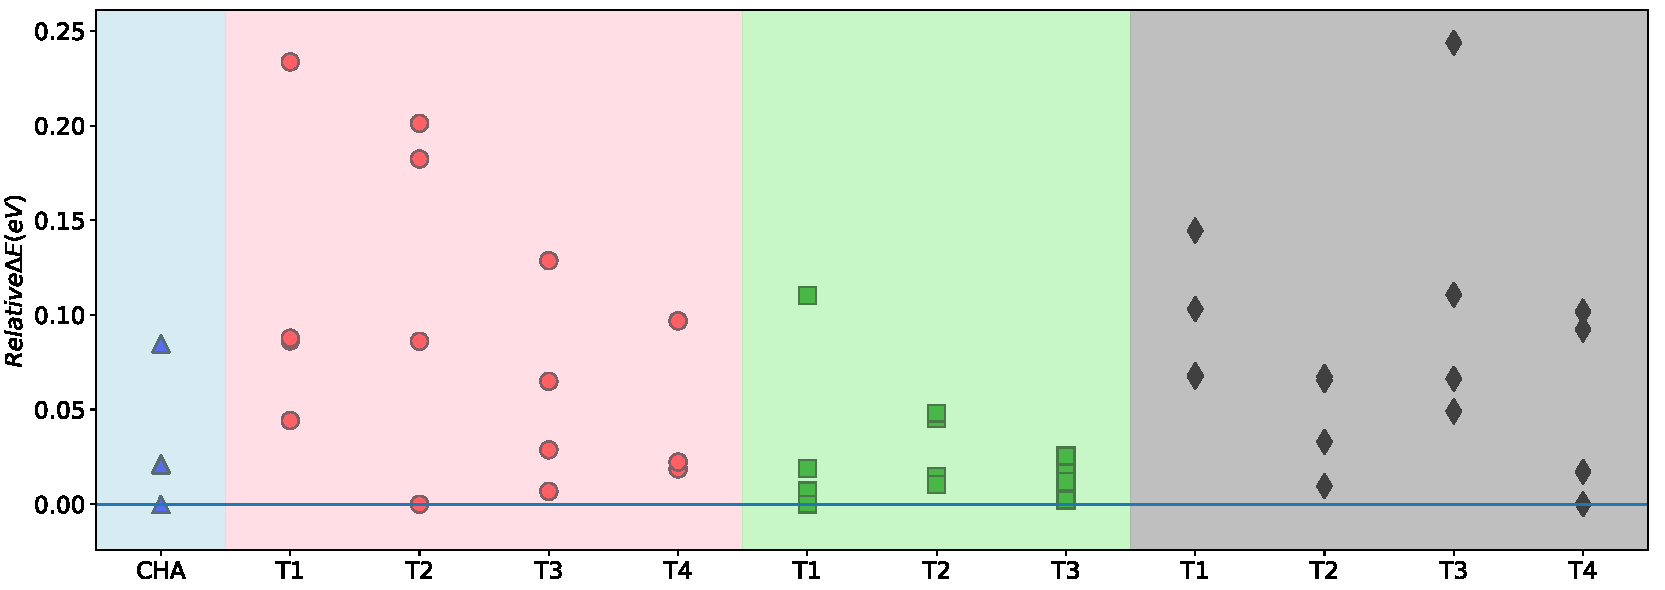
\includegraphics[width=5.2in]{./Figures/Figure-1}
  \caption{ZH exchange energies for (), (), (), ()}
\end{figure}

\begin{enumerate}[resume]
\item The ZCuOH exchange energies and siting locations
\end{enumerate}

\begin{figure}[H]
\centering
  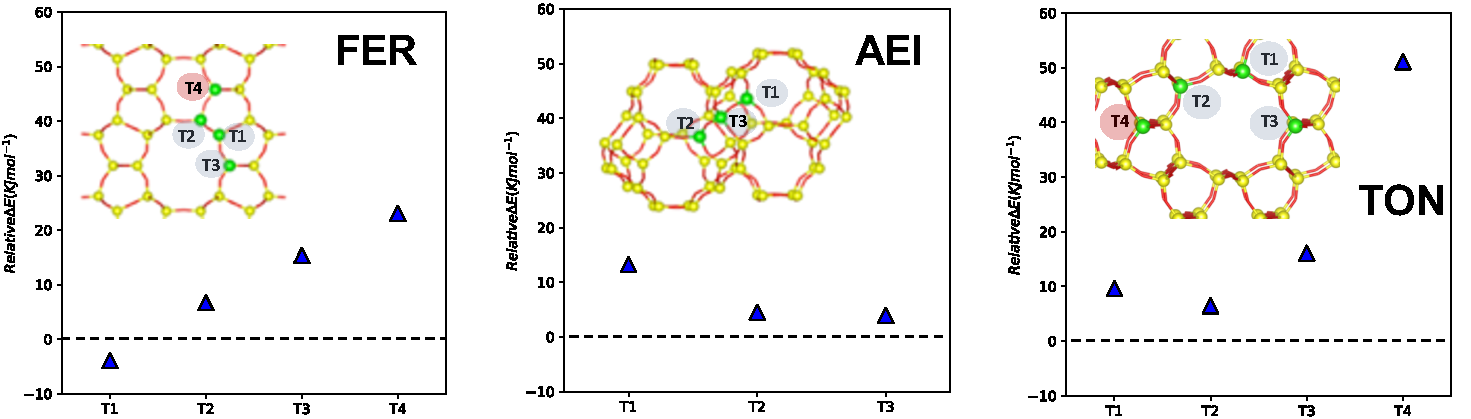
\includegraphics[width=5.2in]{./Figures/Figure-2}
  \caption{Relative ZCuOH exchange energies  for (), (), () compared to CHA.}
\end{figure}


\begin{enumerate}[resume]
\item The Z2H2 exchange energies and siting locations
\end{enumerate}
\begin{enumerate}[resume]
\item The Z2Cu exchange energies and siting locations
\end{enumerate}
\begin{enumerate}[resume]
\item The Z2Cu and ZCoOH exchange
\end{enumerate}
\begin{enumerate}[resume]
\item The Z2Cu site counting
\end{enumerate}
\begin{enumerate}[resume]
\item The compositional phase diagrams
\end{enumerate}

\begin{figure}[H]
\centering
  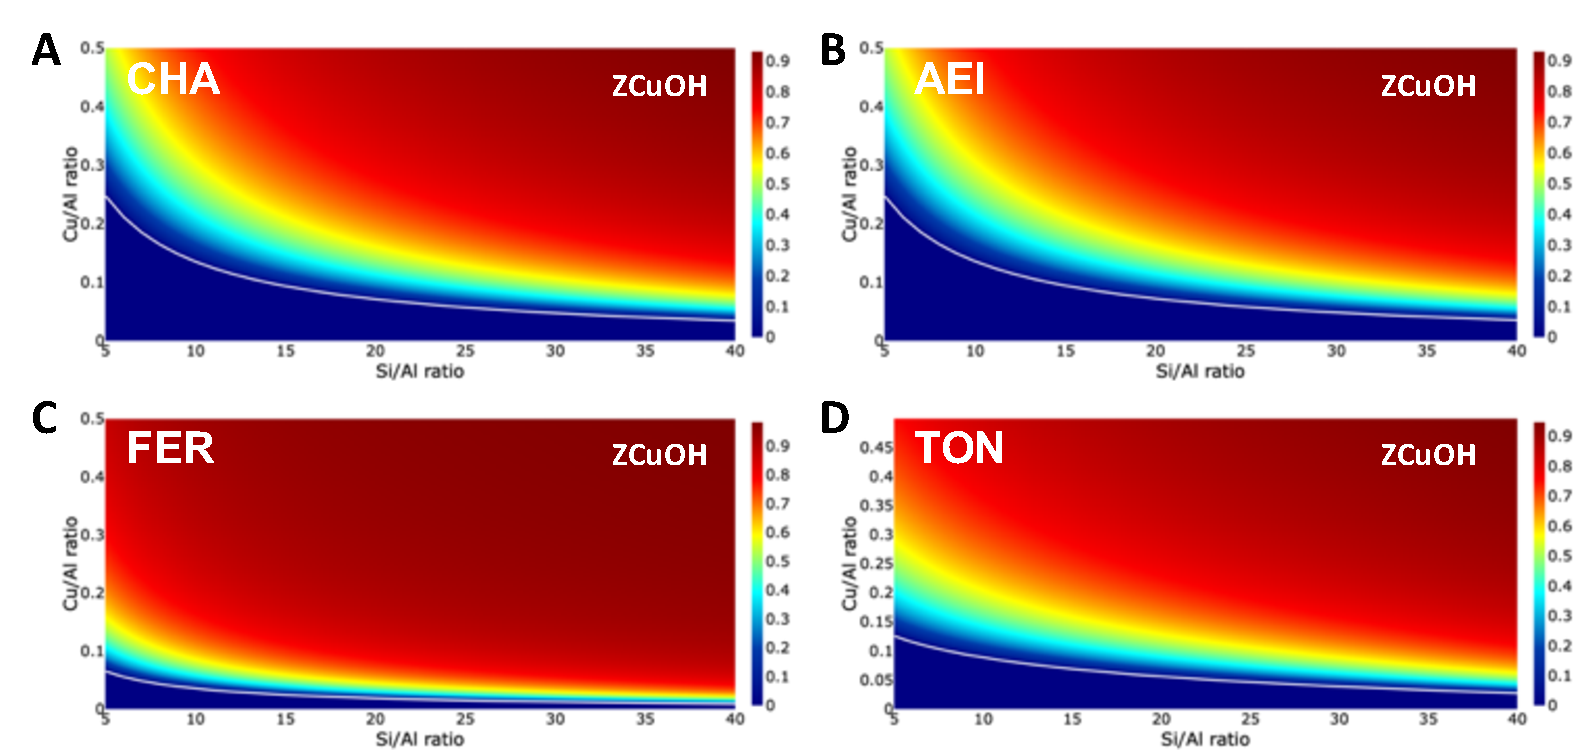
\includegraphics[width=5.2in]{./Figures/Figure-5}
  \caption{Compositiona phase diagrams for (), (), (), ()}
\end{figure}


\subsection*{Conclusions}

In this work, we interrogate and compare Cu+ ion pairability in zeolites through statistical modeling and Monte Carlo simulation, and identify the sensitivity of the pairable Cu+ fraction to the zeolite topology, which promises the potential of rational choice of zeolite topology to tailor the Cu+ pairing during SCR oxidation half-cycle. This approach can be extended to calculate the Cu+ ion pairability of all 237 zeolite topologies for specific SCR applications of interest. 

\subsection*{References}
\bibliography{Ref}{}
\bibliographystyle{plain}


\end{document}
